\chapter{Experimental Setup} \label{chap:testbed}

The purpose of this chapter is to present the 3D printing robot system used as the testbed. The robotic system consists of a UR5 robot manipulator, 3D print head, and a laser scanner -- each will be described in Section~\ref{sec:ur5}. In Section~\ref{sec:current_work}, we will discuss the previous works done on the robotic system. This includes the system identification model and the \ac {MPC} controller. Finally, based on the errors, we will formalize the hypothesis in Section~\ref{sec:hypo}.
\section{The 3D Printing Robot System} \label{sec:ur5}
\subsection{UR5 Robot Arm} \label{subsec:ur5}
UR5 is a lightweight, flexible industrial robot from Universal Robots. The robot is chosen due to its human-safe operation with a quite good repeatability of 0.1 mm \cite{UR5}. The robot is a serial link 6 \ac{DoF} manipulator with internal controller to take care of the gravity compensation and most of the non-linearities. In general, the robot can be controlled like a system of 6 decoupled servos, although this is only correct to some degree. We will see later why this is the case. Since the internal controller can not be "seen", let alone modified, the UR5 and the controller are viewed as one system. 

The \ac {RL} controller will be implemented in MATLAB which communicates with the UR5 using a TCP/IP protocol on 125 Hz frequency. There is a number of ways to send control command to the robot:
\begin{enumerate}
\item Tool position commmand \\
The tool position means the position of the robot's end effector in Cartesian coordinate. The origin of the Cartesian frame is exactly at the robot's base. Figure~\ref{fig:UR5_Robot01} shows a full posture of the UR5 robot. With this type of control input, one can command the end effector to move to a specified tool position $ s = (x, y, z) $ in mm. This type of command results in a smooth motion if applied in a long sampling period (> 1 second). For the 125 Hz communication rate, however, it suffers from a poor jitter.

\item Tool speed command \\
The tool speed command is in the same coordinate as the position command, but now the control input is the velocity of the end effector in mm/s. This command results in a much smoother motion compared to position command.

\item Joint position command \\
This command controls the joint position of individual robot's joint to a specified angle in radian. Similar to tool position command, it results in a jerky motion. 

\item Joint speed command \\
This command drives the individual joint into the desired joint velocity in the unit of radian/s. This results in the smoothest motion compared to others. Due to this reason, this command will be used to drive the robot throughout the thesis.

\begin{figure}
\centering
\includegraphics[width=0.5\linewidth]{UR5_Robot01}
\caption{The UR5 Robot (photo courtesy of Universal Robots)}
\label{fig:UR5_Robot01}
\end{figure}
 
\end{enumerate}

\subsection{Laser Scanner}
The laser scanner is a scanCONTROL 2700-25 series laser manufactured by Micro-Epsilon and mounted on the robot's end effector. It offers a 100 Hz profile frequency, up to 64,000 measuring points per second and 4 $ \mu $m scanning resolution. The laser scanner is used to generate the 3D point cloud of the surface we would like to print on and to measure the tracking accuracy. Figure~\ref{fig:scanCONTROL} shows the 3D view of the laser scanner.

\begin{figure}
	\centering
	\includegraphics[width=0.5\linewidth]{scanCONTROL}
	\caption{scanCONTROL 2700 series laser scanner (photo courtesy of Micro-Epsilon)}
	\label{fig:scanCONTROL}
\end{figure}

\subsection{3D Print head}
The 3D print head is a Cobalt C29 inkjet printhead developed by Oc{\'e} Technologies B.V.  Since the print head does not contribute to the controller design and implementation, it will not be used throughout the thesis. Figure~\ref{fig:ur5-endeffector} shows the robot's end effector with print head attached \cite{sunniva2013}.


\begin{figure}
\centering
\includegraphics[width=0.5\linewidth]{ur5}
\caption{The end effector of the UR5 robot with 3D print head and laser scanner attached (photo courtesy of Sunniva Ipenburg)}
\label{fig:ur5-endeffector}
\end{figure}

\section{Previous Work} \label{sec:current_work}
In this section, we will present a short overview of the previous works done by de Gier from \ac {DCSC}, specifically on the system identification and the \ac {MPC} controller \cite{Gier2013}.

\subsection{System Identification}
An important assumption for the identification is that the robot acts as six decoupled servos along with their internal controller. Additionally, it is also assumed that each joint is a \ac{LTI} system. This implies that there will be six individuals \ac {LTI} model to identify. Each model is a \ac{SIMO} system with the joint velocity reference $\dot{\theta}_r$ as the input and joint position $\theta$ and velocity $\dot{\theta}$ as the outputs. 

For this purpose, a subspace identification method is used. According to the significant singular values, the order of each model is determined to be either 4 or 5 \cite{verhaegen2007filtering}. After the models are obtained, each joint model is then validated using a square input signal while the other joint angles are held constant. The \ac{VAF} values of each joint for the validation test is shown in Table~\ref{tab:vaf}. Although the result shows a quite good \ac {VAF} score, it is still not good enough to achieve a perfect tracking. To give an example of the performance, the model validation plot of joint 1 and 5 is shown in Figure~\ref{fig:idenJoint}.

\begin{table}
\caption{\ac {VAF} scores of the simulated outputs for all joints}	
	\centering
	\begin{tabular}{|c|c|c|}
		\hline Joint & Position  & Velocity \\ 
		\hline 1 & 98.64 & 87.33 \\ 
		\hline 2 & 98.05 & 88.33 \\ 
		\hline 3 & 98.55 & 88.47 \\ 
		\hline 4 & 98.97 & 89.50 \\ 
		\hline 5 & 99.46 & 90.32 \\ 
		\hline 6 & 98.87 & 85.13 \\ 
		\hline 
	\end{tabular} 
	\label{tab:vaf}
\end{table}


\begin{figure}
	\centering
	\begin{subfigure}[b]{0.4\textwidth}
		\includegraphics[width=1\linewidth]{"../../Progress Report/Joint5"}
		\caption{}
		\label{fig:Joint5}
	\end{subfigure}%
	~ %add desired spacing between images, e. g. ~, \quad, \qquad, \hfill etc.
	%(or a blank line to force the subfigure onto a new line)
	\begin{subfigure}[b]{0.4\textwidth}
		\includegraphics[width=1\linewidth]{"../../Progress Report/Joint1"}
		\caption{}
		\label{fig:Joint1}
	\end{subfigure}
	\caption{Model validation of joint 1 and 5 for joint position and velocity}\label{fig:idenJoint}
\end{figure}

\newpage
\subsection{\ac{MPC} Controller}
The previous work involves a design and implementation of \ac {MPC} controller. As the comparisons, we will control the robots using 3 of the 4 methods described in Subsection~\ref{subsec:ur5}: tool position, tool velocity and joint velocity command. We will call these three control methods the default controllers. The experiment is to make the robot following a straight line along X-axis with constant values on Y and Z axes.  In order to see the effect of robot's speed to the errors, the experiment is repeated with three different speeds for the default controllers. As for the \ac {MPC}, only one speed is possible due to the difficulty to modify the provided \ac {MPC} program. The plots for Y and Z trajectories are shown in Figure~\ref{fig:trajectory_data_Y} and \ref{fig:trajectory_data_Z} respectively. 

As we can see, there is a shaky behavior in both axes trajectories. To have an idea of how large the amplitude of the jitter, we calculate the difference between maximum and minimum values of each trajectory as shown in Table~\ref{tab:y_jitter} and \ref{tab:z_jitter}. The Y-axis trajectory for the default controllers are slowly drifting from the desired value. This is expected since the default controllers are basically open loop controllers. This causes the jitter's amplitude to be much higher than the \ac {MPC} (see Table~\ref{tab:y_jitter}). Furthermore, for different speeds, the jitters of each default controller behave similarly. If we run the controller for several iterations at constant speed, the plot (not shown here) confirms that the jitter indeed shows a repeating behavior. 

Table~\ref{tab:y_jitter} has shown that the \ac {MPC} controller manages to reduce the jitter significantly -- it almost reaches the robot repeatability. However, for The Z-axis trajectory, the jitter is much larger. 

\begin{table}
	\centering
	\caption{The difference between maximum and minimum values of Y-axis trajectory with different control methods}
	\begin{tabular}{|c|c|c|}
		\hline
		Control method & speed & jitter's amplitude (mm) \\
		\hline		
		& $ \times $1 & 0.635678\\
		Tool Position & $ \times $2 & 0.670974\\
		& $ \times $4 & 0.624456\\
		\hline		
		& $ \times $1 & 0.529104\\
		Tool Velocity & $ \times $2 & 0.376090\\
		& $ \times $4 & 0.320906\\
		\hline		
		& $ \times $1 & 0.550691\\
		Joint Velocity & $ \times $2 & 0.522474\\
		& $ \times $4 & 0.490630\\				
		\hline
		\ac {MPC} & $ \times $1 & 0.120889 \\
		\hline

	\end{tabular}
	\label{tab:y_jitter}
\end{table}

\begin{table}
	\centering
	\caption{The difference between maximum and minimum values of Z-axis trajectory with different control methods}
	\begin{tabular}{|c|c|c|}
		\hline
		Control method & speed & jitter's amplitude (mm) \\
		\hline		
		& $ \times $1 & 0.879843\\
		Tool Position & $ \times $2 & 0.805172\\
		& $ \times $4 & 0.800554\\
		\hline		
		& $ \times $1 & 0.904581\\
		Tool Velocity & $ \times $2 & 0.909465\\
		& $ \times $4 & 1.007834\\
		\hline		
		& $ \times $1 & 0.793960\\
		Joint Velocity & $ \times $2 & 0.795276\\
		& $ \times $4 & 0.975885\\				
		\hline
		\ac {MPC} & $ \times $1 & 0.795315 \\
		\hline
		
	\end{tabular}
	\label{tab:z_jitter}
\end{table}

%\begin{figure}
%\centering
%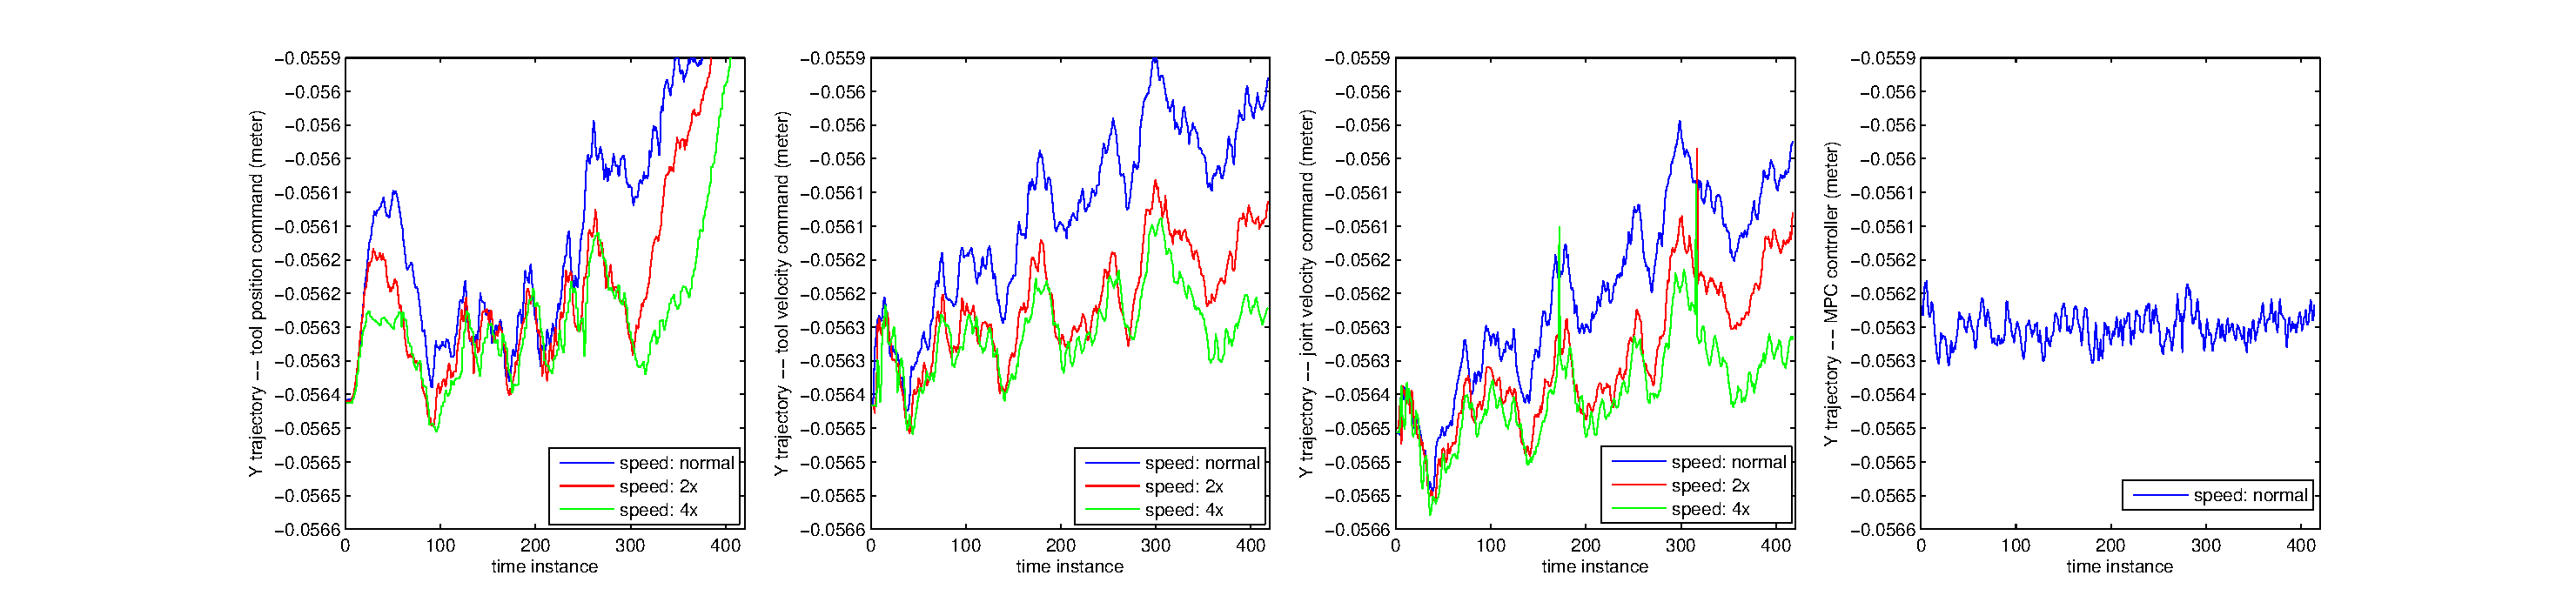
\includegraphics[width=0.7\linewidth]{trajectory_data_Y}
%\caption{the Y trajectories of the robot with different controllers. From left to right: tool position command, tool velocity command, joint velocity command and \ac{MPC}}
%\label{fig:trajectory_data_Y}
%\end{figure}
%\begin{figure}
%\centering
%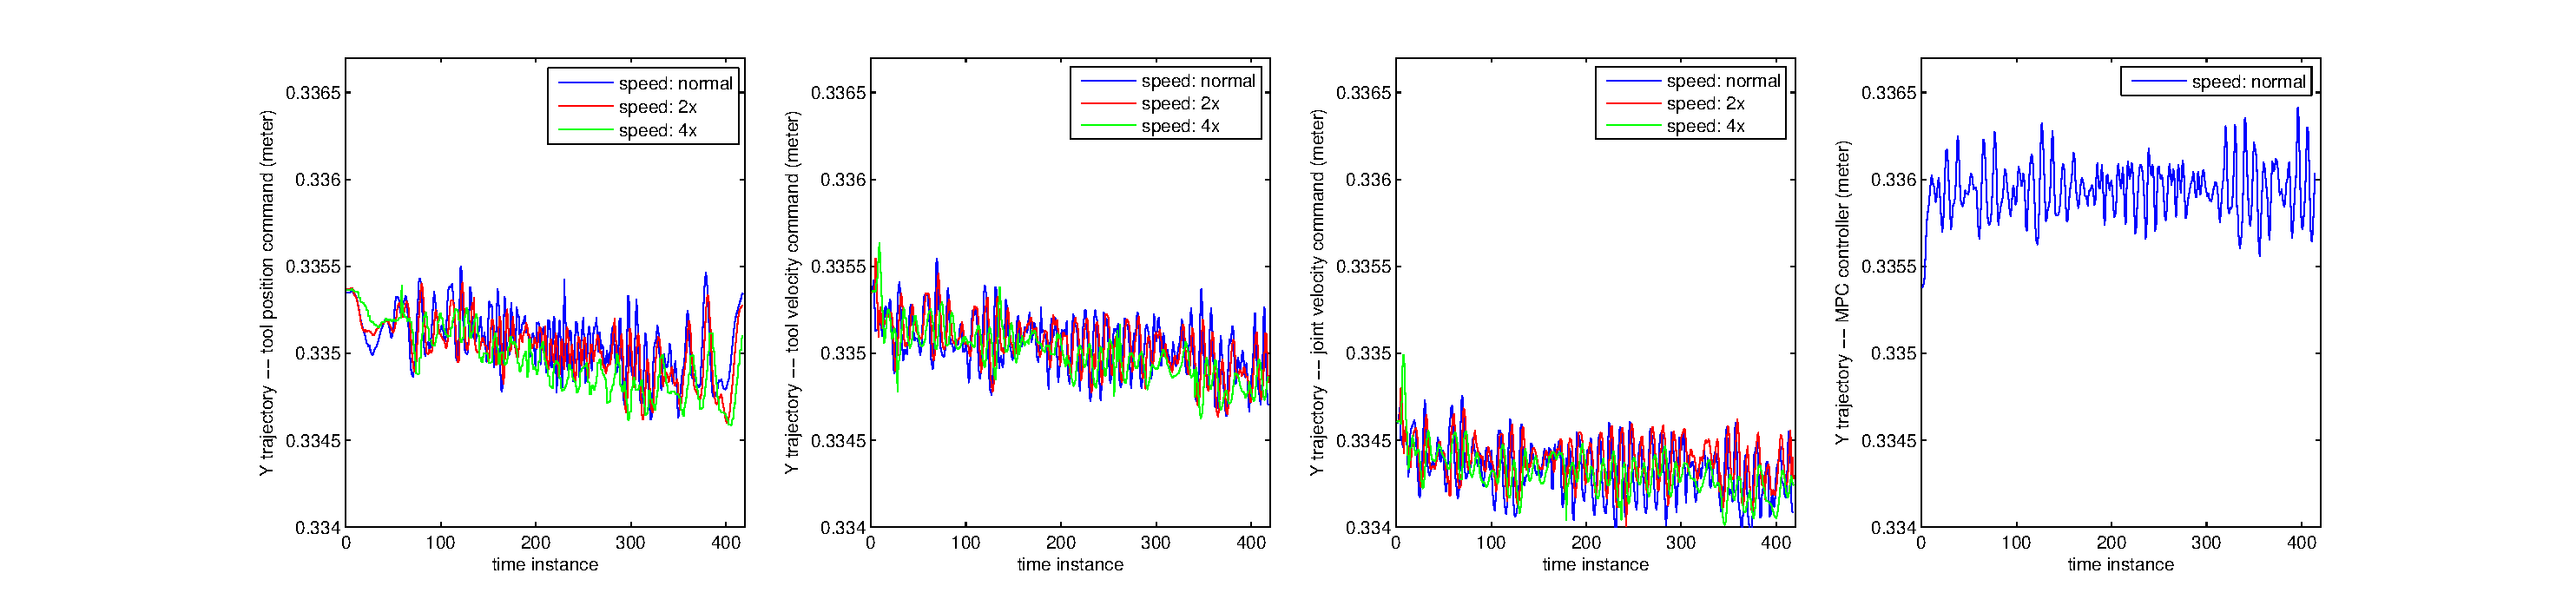
\includegraphics[width=0.7\linewidth]{trajectory_data_Z}
%\caption{the Z trajectories of the robot with different controllers. From left to right: tool position command, tool velocity command, joint velocity command and \ac{MPC}}
%\label{fig:trajectory_data_Z}
%\end{figure}

 

